\section{Tiered Compilation in Hotspot}
\label{sec:tiered}
As mentioned in the introduction, Programming Language Virtual Machines like Java Hotspot feature a multi-tier system when compiling methods during execution. 
Java VM's typically use Java Bytecode as input, a platform independent intermediate code generated by a Java Compiler like \texttt{javac}.
The Bytecode is meant to be interpreted by the virtual machine or further compiled into platform dependend machine code.
Hotspot includes one interpreter and two different compilers with different profiling levels resulting in a total of 5 different levels. The following Figure \ref{fig:hs_tiers} gives a short overview as well as showing the standard transitions.
\begin{figure}[h]
  \begin{center}
    \centering
    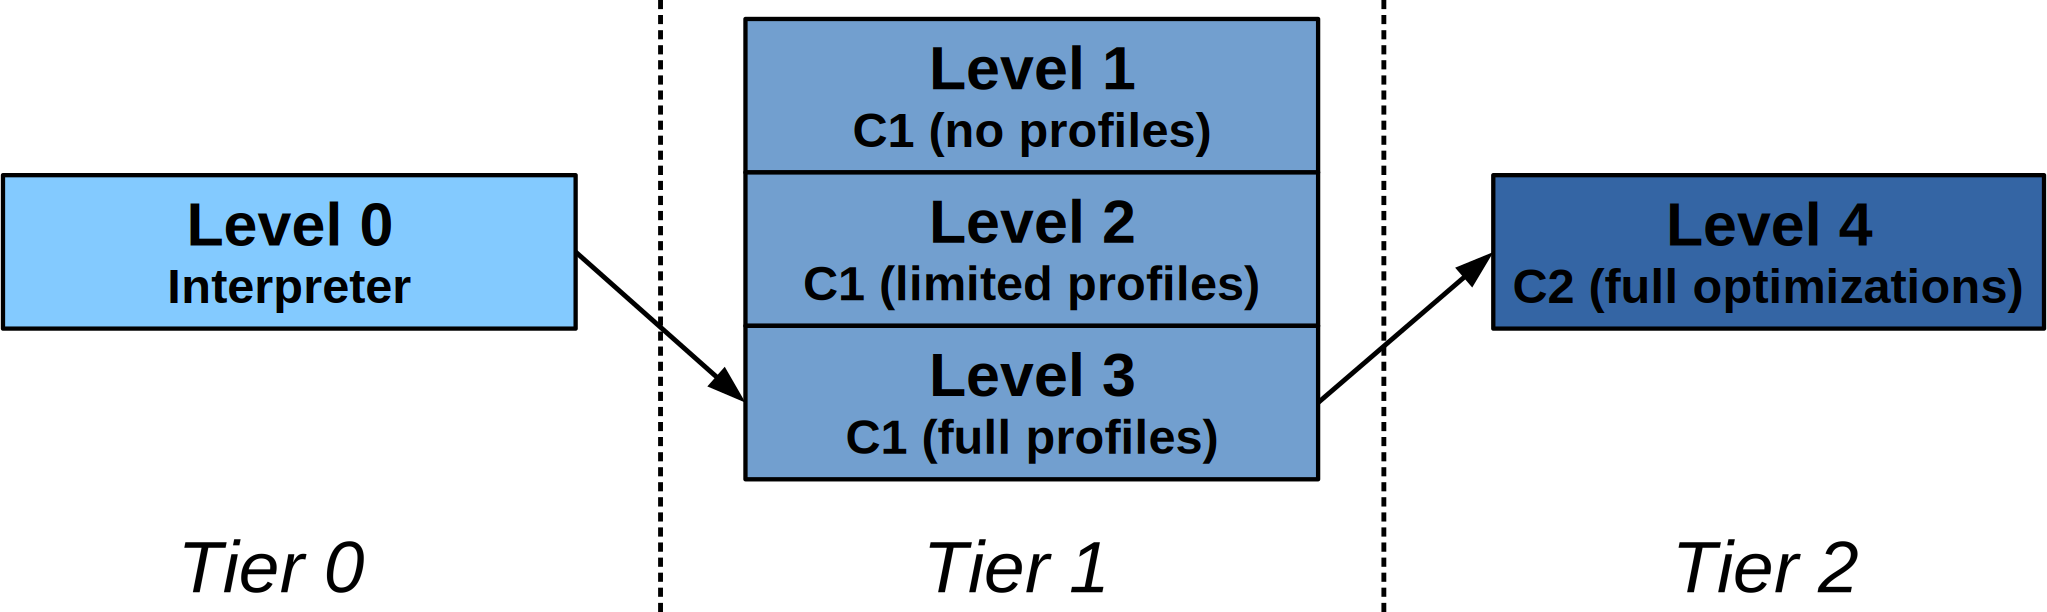
\includegraphics{figures/hs_tiers.png}
    \caption{Overview over compilation tiers}
    \label{fig:hs_tiers}
  \end{center}
\end{figure}

All methods start being executed by Tier-0 also called the Interpreter.
The interpreter is template-based meaning for each bytecode instruction it emits a predefined assembly code snippet.
During execution this code is also profiled. This means method execution counters and loop back-branches and additional statistics are counted. Once one these counters exceed a predefined, constant threshold the method is further progressed, for example compiled with a higher tier.
\\\\
The standard behavior of Hotspot is to proceed with Level 3 (Tier 1). This means the method gets compiled with C1, also referred to as \textit{client} compiler, and continues gathering full profiles.
C1's goal is to provide a fast compilation with a low memory footprint.
The client compiler performs simple optimizations such as constant folding, null check elimination and method inlining.
More information about C1 can be found in \cite{client_compiler_talk} and \cite{client_compiler}.
The levels 1 and 2 include the same optimization but offer no or less profiling information.
\\\\
Eventually, when further compile thresholds are exceeded, the JVM further compiles the method with C2, also known as \textit{server} compiler.
The server compiler makes use of the gathered profiles in Tier 0 and Tier 1 and produces highly optimized code. C2 includes far more optimizations like loop unrolling, common subexpression elimination and elimination of range and null checks. It performs optimistic method inlining, for example by converting some virtual calls to static calls.
A more detailed look at the server compiler can be found in \cite{server_compiler}.
\\\\
The naming scheme \textit{client/server} comes from back in the days were tiered compilation was not available and one had to choose the compiler via a Hotspot command line flag. The \textit{Client} compiler was meant to be used for interactive client programs with graphical user interfaces where response time is more important than peak performance. For long running server applications, the highly optimized but slower server compiler was used. 
\\\\
Tiered compilation was introduced to improve start-up performance of the JVM.
Starting with the interpreter means that there is zero wait time until the method is executed since one does not need to wait until a compilation is finished. C1 allows the JVM to have more optimized of the code available early which then can be used to create a richer profile to be used when compiling with C2. Ideally this profile already contains most of the program flow so less deoptimizations (see \ref{sec:deoptimizations} occur.

\section{On Stack Replacement}
\label{sec:onstackreplacement}
At some point during interpretation or just-in-time compilation a method's code might need to be replaced by a higher tier compiled method. This happens for example when a method is interpreted and a version compiled with C1 is ready.
Instead of waiting for the next method invocation Hotspot can replace the method directly on the stack while it is still running (see Figure \ref{fig:osr}).
This is usually done when the JVM realizes that the method contains a long running loop by counting the back branches.
\begin{figure}[h]
  \begin{center}
    \centering
    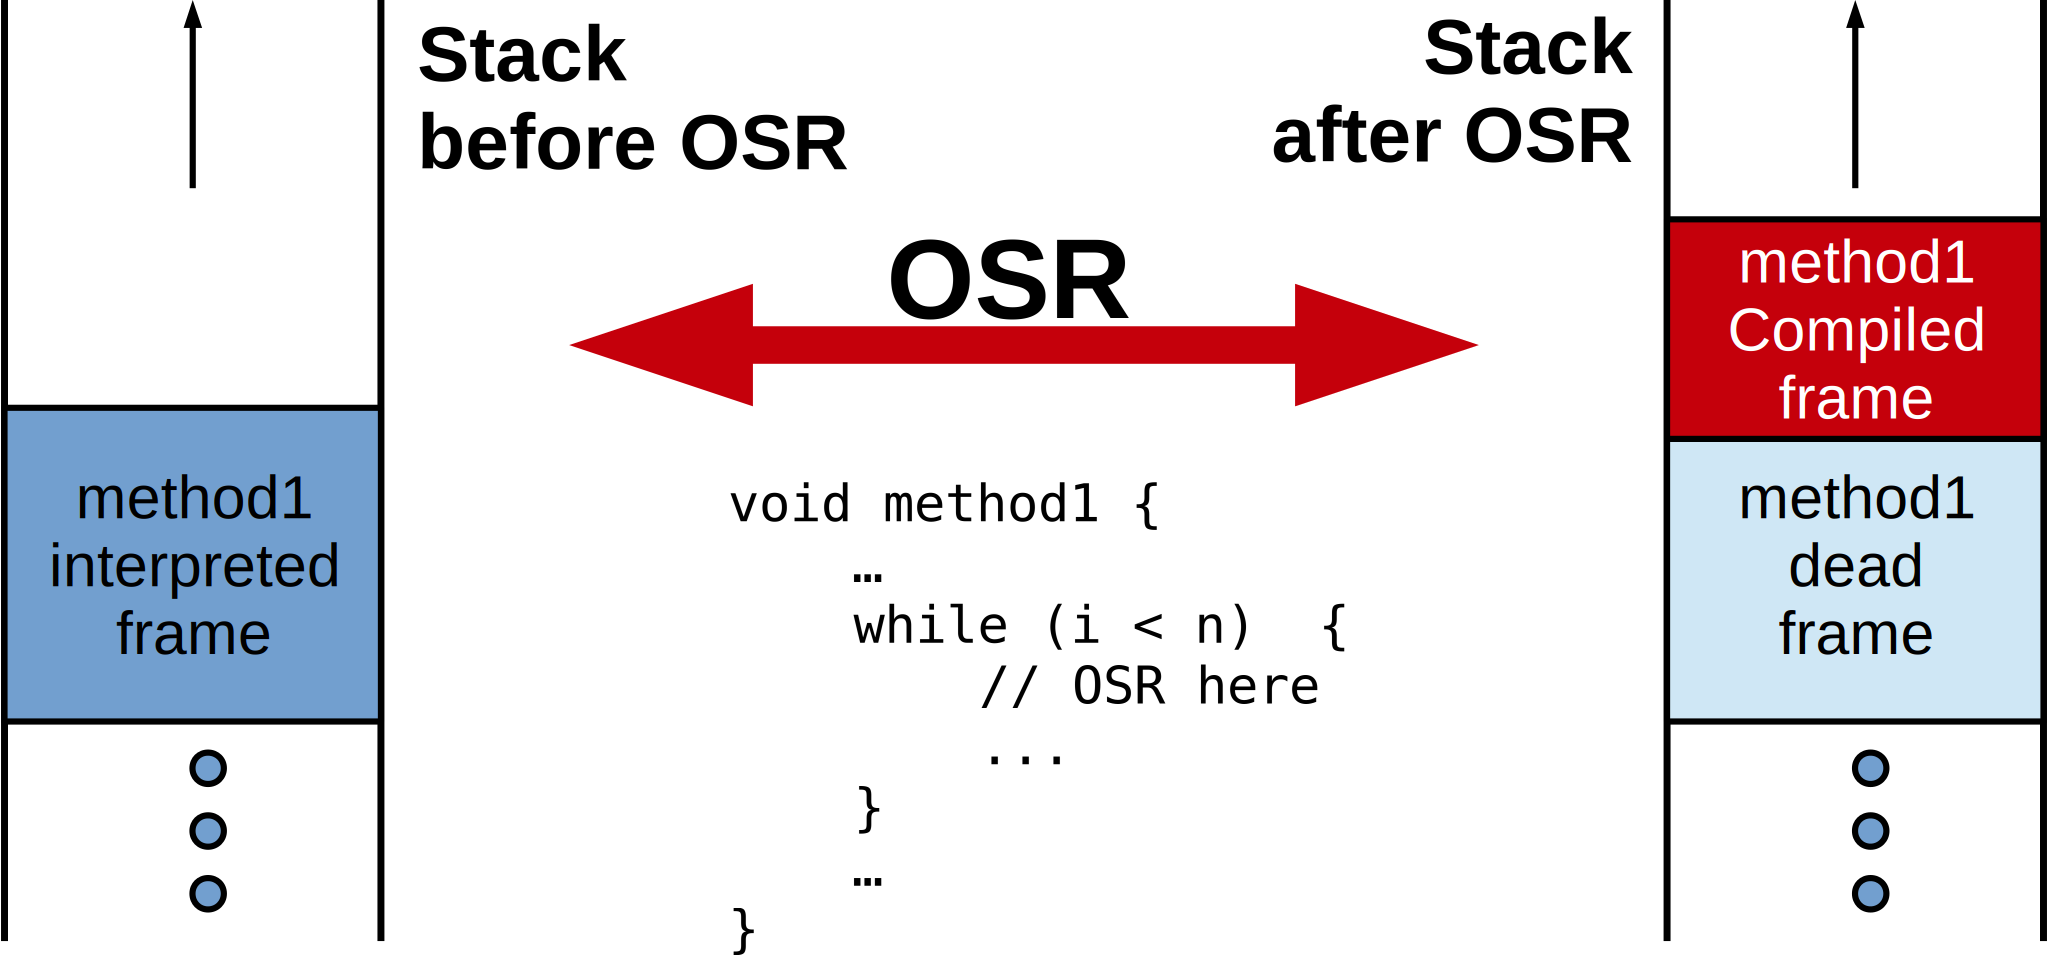
\includegraphics{figures/osr.png}
    \caption{Overview over compilation tiers}
    \label{fig:osr}
  \end{center}
\end{figure}

\section{Deoptimizations}
\label{sec:deoptimizations}

\section{Compile Thresholds}
\label{sec:compilethresholds}

\section{Examples}
\label{sec:examples}
